\documentclass{beamer}
\usepackage{siunitx}

\usepackage[utf8]{inputenc}
\usepackage{amsmath}

\newcommand{\myvec}[1]{\ensuremath{\begin{pmatrix}#1\end{pmatrix}}}
\usetheme{Berlin}
\title{MATRIX PROJECT - Q33}
\author{BHAVYA BAGLA (CS17BTECH11007) \newline CHANDER SHEKHAR (CS17BTECH11011) }


\begin{document}

\maketitle
\begin{frame}{QUESTION:}
\item A circle passes through 
\begin{equation}
A =\myvec{-2\\ 4} 
\end{equation} 
and touches the $y$-axis at 
\begin{equation} 
B =\myvec{0\\ 2}. 
\end{equation}
Which one of the  following equations can represent a diameter of this circle?
\begin{enumerate} 
\item $\myvec{4 & 5}\vec{x} = 6 $
\item $\myvec{2 & -3}\vec{x} +10 = 0 $
\item $\myvec{3 & 4}\vec{x} = 3 $
\item $\myvec{5 & 2}\vec{x} +4= 0 $
\end{enumerate} 


\end{frame}
\begin{frame}{}
    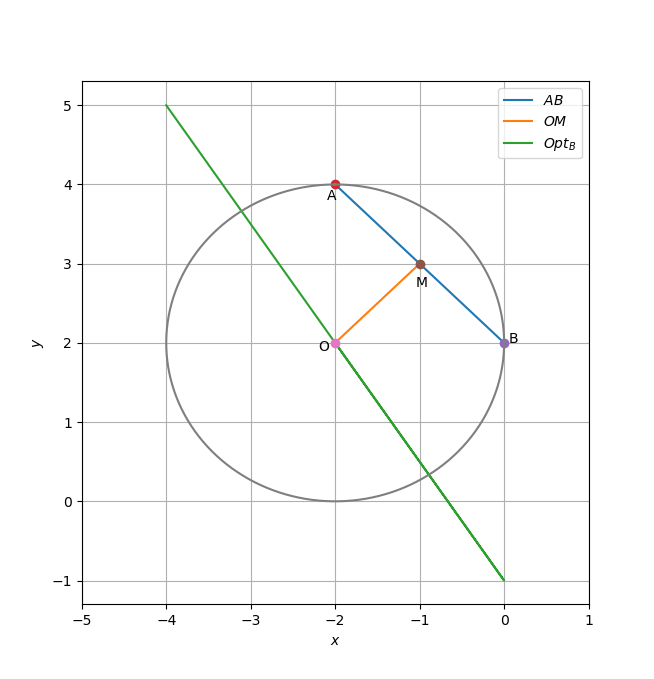
\includegraphics[scale=0.5]{Q_33_Graph.png}
\end{frame}
\begin{frame}{SOLUTION :}
First, we compute direction vector of line passing through given two points using matrix it comes out to be 
\newline 
\begin{equation}
    Direction Vector = T = \myvec{-1\\1}
\end{equation}
\newline
Now, we compute perpendicular bisector of this line segment \textbf{AB} using its mid point and direction vector of AB =\textbf{T}(it is equivalent to normal vector of the perpendicular bisector)  \newline

%\begin{equation}
 %   Normal Vector = N = \myvec{1\\1}
%\end{equation}


\begin{equation}
    Mid Point = M = \myvec{-1\\3}
\end{equation}
\end{frame}


\begin{frame}{SOLUTION:}
Equation of perpendicular bisector:\newline

\begin{equation}
    T^T X = p
\end{equation}

To compute value of p we put X equal to M in the above equation.
\newline

\begin{equation}
    T^T M = p
\end{equation}

\begin{equation}
        \myvec{-1&1}\myvec{-1\\3}=p
\end{equation}
\begin{equation}
    p=4
\end{equation}

\end{frame}

\begin{frame}{Solution: }

Final Equation of perpendicular bisector,
\begin{equation}
        \myvec{-1&1}\vec{x} = 4 
\end{equation}

As the circle touches the y-axis at (0,2) then circle should lie on the line

\begin{equation}
        y=2
\end{equation}
which can be represented in the following way using matrices

\begin{equation}
        \myvec{0&1} \vec{x} = 2
\end{equation}


\end{frame}

\begin{frame}{Solution: }
    The intersection of these two lines (9) and (11) is the center because both these lines pass through center.\newline
    
\begin{equation}
        Center= O =\myvec{-2\\2}
\end{equation}

Now whichever line given in options passes through the center \textbf{O}, is the answer. 
\end{frame}

\begin{frame}{Solution: }
\item \textbf{1: }$\myvec{4 & 5}\vec{x} = 6 $ 
\begin{equation}
    \myvec{4 & 5}\myvec{-2\\2} \neq 6
\end{equation}


\item \textbf{2: }$\myvec{2 & -3}\vec{x} +10 = 0 $
\begin{equation}
    \myvec{2 & -3}\myvec{-2\\2} +10 = 0 
\end{equation}
As L.H.S is equal to R.H.S.,this answer is correct.
\end{frame}
\begin{frame}

\item \textbf{3: }$\myvec{3 & 4}\vec{x} = 3 $

\begin{equation}
    \myvec{3 & 4}\myvec{-2\\2} \neq 3 
\end{equation}


\item \textbf{4: }$\myvec{5 & 2}\vec{x} +4= 0 $
\begin{equation}
    \myvec{5 & 2}\myvec{-2\\2} +4 \neq 0 
\end{equation}
Line represented in $2^{nd}$ option is one of the diameters of the given circle

\end{frame}
\section{Introduction}

\end{document}
